\section{Detection and Time Synchronization}
\label{sec:detection}

As illustrated in Figure~\ref{fig:sig_acquis_chain}, the first step to analyze
the signal acquisition chain is to formulate the detector.
The detection algorithm proceeds sequentially and each step a window of length $N$ received samples with 
$N{-}1$ overlapped samples of the previous window is considered. The sequential detection problem solved 
in this paper is fundamentally equivalent to sequential frame synchronization~\cite{Massey_72,Lui_Tan_86,Scholtz_80}.
To make analysis easier, we will focus on deriving the detection algorithm   
by assuming the fractional delay is neglected at a sufficiently high sample rate in this section.
The effect of fractional delay on our proposed detection algorithm will be discussed with different sampling rate, or equivalently, 
oversampling factor in simulation section (Section~\ref{sec:simulations}). 

\begin{figure}[t]
  \centerline{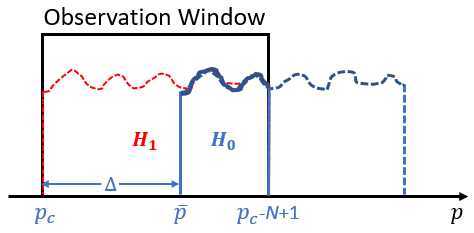
\includegraphics[width=2.4in]{H1_H0_hypothesis.png}}
  \caption{Received sequence in observation window (the shaded area) containing partial preamble (Blue: current received sequence. Red: received sequence at true delay $\bar{p}$)}
  \label{fig:H1_H0_hypothesis}
  \end{figure}

We start by looking at the likelihood ratio test (LRT) for the detection task:
Let $H_0$ be the null hypothesis that the preamble is not completely presented in the received sequence from the obeservation window 
against the alternative $H_1$ that it does. 
Define $\Delta$ to be the distance between current received sequence at position $p_c$ and the true position ($\bar{p}$) of the preamble, 
i.e., $\Delta=|\bar{p}-p_c|$. Figure~\ref{fig:H1_H0_hypothesis} illustrates the case that the received sequence in observation window contains partial preamble.
It is symmetric if the partial preamble shows on the left side of the observation window ($p_c>\bar{p}$).
It is obvious that under $H_0$, $\Delta \neq 0$ while $H_1$ means $\Delta=0$. 
Based on~\eqref{eq:model}, the conditional likelihood ratio test (LRT) can be built 
between $H_0$ and $H_1$ by given the distance $\Delta$, the phasor $S{=}Ae^{j\phi}$ and frequency offset $b{=}e^{j2\pi \delta}$
at true delay $\bar{p}$ (under $H_1$),

\begin{equation}
    \label{eq:likelihood ratio}
    \begin{aligned}
    &\Lambda(R|S,b,\Delta)=\frac{p_{R|H_1,S,b}(r|H_1,S,b)}{p_{R|H_0,S,b,\Delta}(r|H_0,S,b,\Delta)}= \\
    &\frac{\displaystyle \prod_{n=0}^{N-1}\frac{1}{\sqrt{\pi N_0}}\exp{(-\frac{1}{2}\frac{|r_{n}{-}s_nSb^n|^2}{N_0/2})}}
    {(\displaystyle \frac{1}{\sqrt{\pi N_0}})^N\displaystyle \prod_{n=\Delta}^{N-1}\exp{(-\frac{1}{2}\frac{|r_{n}{-}s_{n-\Delta}Sb^{n-\Delta}|^2}{N_0/2})} 
    \displaystyle \prod_{n=0}^{\Delta-1}\exp{(-\frac{1}{2}\frac{|r_n|^2}{N_0/2})}} \\
    &\LRT{H_1}{H_0} \eta.
    \end{aligned}
\end{equation}
Cancelling the common parts and taking the logarithm,~\eqref{eq:likelihood ratio} is reduced to

\begin{equation}
    \label{eq:log likelihood}
    \begin{aligned}
    \Re\Bigg\{\sum_{n=0}^{N-1}r_{n}s^*_nS^*b^{-n}-
    \sum_{n=\Delta}^{N-1}r_{n}s^*_{n-\Delta}S^*b^{-(n-\Delta)}\Bigg\}
    &\LRT{H_1}{H_0} \frac{N_0}{2}\ln\eta \\
    &+\frac{A^2}{2}\sum_{n=N-\Delta}^{N-1}|s_n|^2.
    \end{aligned}
\end{equation}
The second summation on the left hand side points to the inner product of the overlap between
the observed (partial) preamble and the true preamble. 
To put it another way,~\eqref{eq:log likelihood} says that the likelihood 
ratio test reduces to the difference between full cross-correlation and overlapped cross-correlation
of received and reference sequences. However, note that in practice, the overlapped cross-correlation is not possible to be
precomputed while detection since $\Delta$ is always an unknown information to the receiver.
Fortunately, if we move it to the right hand side, the reduction by cross-correlation can be reflected by the threshold.
Thus, based on above discussion, after some proper scaling, the LRT finally reduces to a generalized correlation function in terms of the time instant (delay) $p$,

\begin{equation}
    \label{eq:generalized_corr}
    \rho(p)=
    \frac{\Re\{\langle
      \bm{r}_{p},\hat{\bm{s}}_{p}\rangle\}}
    {||\bm{r}_{p}||\cdot||\hat{\bm{s}}_{p}||} \LRT{H_1}{H_0} \gamma
  \end{equation}
where $\hat{\bm{s}}_{p}$ represents the carrier-estimate corrected preamble, i.e., $\hat{s}_{p}[n]~{=}~s_{n}\hat{S}_{p}\hat{b}_{p}^n$ for $n=0,\ldots,N{-}1$,
at delay $p_c$. $\hat{b}_{p_c}$ and $\hat{S}_{p_c}$ are the frequency and phasor estimates at delay $p$.
$||\bm{r}_{p}||$ is the Euclidean norm of received data sequence at delay $p$.
$\gamma$ is the normalized detection threshold which lies on the range of $[0,1]$.
Note, the LRT in~\eqref{eq:likelihood ratio} is not practical since the frequency and phasor offsets at true delay $\bar{p}$
is unknown while detection except for the distance $\Delta$. 
Thus, instead of LRT, a generalized likelihood ratio test (GLRT) based detector is built relying on frequency and phasor estimates from each window of received sequence;
To get $\hat{b}_{p_c}$ and $\hat{S}_{p_c}$,
recall the LRT of~\eqref{eq:likelihood ratio} is built conditionally on known frequency and phase offset 
at true position of the preamble; Therefore, the algorithm of computing the frequency and phase estimates at $p_c$ 
can be also by assuming the current received sequence contains the complete true preamble.
% this tells the reason why we do estimation by assuming the position of preamble is known.

In conclusion, a GLRT based detector of~\eqref{eq:generalized_corr} is derived for detection in this paper, and it relies on the frequency and phase estimates of the observed sequence.
Furthermore, since the sequential detection proceeds at every time instant, to make it work in practice, the complexity of the carrier estimates becomes
much crucial. A low computational-complexity estimator should be derived for real detection purpose.

% should not include the original fractional delay part since I don't know the meaning for introducing the expected loss.
% I think to talk about how large of the oversampling factor that the effect of fractional delay can be neglected is meaningful but not deep.







